% !TEX root = ../main.tex

% Mini-project section

\section{Mini-project}
\subsection{Proposal}
In constrained Bayesian optimization (CBO), the goal is to maximize an expensive objective function
subjected to a number of constrains using Bayesian optimization. To accomplish this goal, one needs to construct an optimization policy that takes into account the constraints and favors the input region satisfying them, i.e. the feasible region. An interesting topic is how to adjust the level of favoritism for feasible points as infeasible points can still be useful by providing information about the behaviours of
the feasible region. In this project, these adjustments are encoded into the policy by relaxing or tightening the original constraints.

To include the feasibility of constrains in their policies, \cite{gardner2014bayesian,gelbart2014bayesian} used the expected improvement acquisition function weighted by the probability of feasibility while \cite{bernardo2011optimization} used a function called integrated expected conditional improvement that computes expected reduction in improvement when a new point is evaluated. \cite{gelbart2014bayesian} also considered the probability of feasibility as the acquisition function but this puts too much preference on finding the feasible region. \cite{eriksson2021scalable} used the total constraint violation to choose the next observations. This, however, is sensitive to scaling and requires a transformation to stabilize the objective and constraints. \cite{kramer2010review} used a fitness value to choose the next point and set the fitness of infeasible points to zero. It is important to note that most methods for CBO encode a fixed notion of preference for feasible points. This eliminates the need for extra hyperparameter tuning but the methods may behave suboptimally compared to ones with varied preference.

In this report, the original CBO problem is augmented by auxiliary parameters that control the looseness of the constraints. With this, I develop a new class of acquisition functions by weighting the notion of utility for these augmented problems. Finally, I propose an adaptive weighting scheme that changes the preference for feasible points based on observed dataset.

The main challenge for this scheme is, of course, how to set the weighting scheme. To do this, one needs to know to what extend changing the scheme would affect the level of favoritism for feasible points and the overall performance of the CBO policy. Too much emphasis on feasibility can lead to the objective not being optimized as quickly while to little emphasis may not yield any feasible points. Another concern is the computational complexities that come with the proposed method. There are elements that vary depending on the auxiliary variable, complicating any integration in the acquisition function. This means the acquisition function may not have a simple closed formula and instead needs to be approximated via sampling.

This project provides an example of how more information about the constraints can be incorporated into the optimization policy by relaxing and tightening the original CBO problem. I believe this approach is an intuitive way of viewing the trade-off between optimizing the objective and satisfying the constraints. In addition, I think the adaptation of this trade-off is a very useful practice in order to improve methods for CBO, similar to how the adaptation of the exploitation-exploration trade-off (e.g. trust region approach \cite{eriksson2019scalable,eriksson2021scalable}) can benefit optimization strategies. 

\subsection{Weighted Constrained Expected Improvement (WCEI)}
\subsubsection{Set up}
Consider the optimization problem
\begin{align}
    \text{Find }x^*=\underset{x\in \Omega}{\text{argmax}}f(x)\text{ s.t. }\textbf{c}(x)\le \textbf{0}
\end{align}
where $f:\Omega\to\bbR,\ c = (c_1,\ldots,c_m),\ c_l:\Omega\to\bbR,l=1,\ldots,m$ are black-box functions, $\Omega\subset \bbR^d$ and
\begin{align}
    \{\textbf{c}(x)\le \textbf{0}\} := \{x:\ c_l(x)\le 0,\ l=1,\ldots,m\}.
\end{align}
The strategy is the same as the one in the set up of the summary section: the objective $f$ and constraints $c_l$ are modelled by a multivariate Gaussian process (GP) surrogate, and at each iteration a policy is used to determine the next observation to add to the dataset until a stop condition is met. For this project, observations of $f$ and $\textbf{c}$ are exact and the policy is to choose an observation maximizing a so-called acquisition function.

\subsubsection{Acquisition function}
Consider the family of augmented CBO problems
\begin{align}
    \text{Find }x^*=\underset{x\in \Omega}{\text{argmax}}f(x)\text{ s.t. }\textbf{c}(x)\le \textbf{a}
\end{align}
where $\textbf{a} = (a_1,\ldots,a_m) \in \bbR^m$ and
\begin{align}
    \{\textbf{c}(x)\le \textbf{a}\} := \{x:\ c_l(x)\le a_l,\ l=1,\ldots,m\}.
\end{align}
When $a_l>0$, the corresponding constraint is relaxed and when $a_l<0$, the constraint is tightened. The \textit{Weighted Constrained Expected Improvement} (WCEI) algorithm I propose uses the following notion of utility
\begin{align}
    u(\calD) = \int\left(\max\limits_{\calD \cap \{\textbf{c}(x)\le \textbf{a}\}} f(x)\right)p(\textbf{a})d\textbf{a}
\end{align}
where $\calD$ is the current dataset and $p$ is the distribution of the auxiliary variable $\textbf{a}$, weighing the utility contribution of each problem in the augmented family. Note that this utility function reduces to that of constrained expected improvement (cEI) \cite{gardner2014bayesian} when $p$ is the point mass at $\textbf{0}$. We can now write the improvement in utility when a new point is added to the dataset
\begin{align}\label{I(x)}
    I(x) := u(\calD')-u(\calD) = \int\max\{f(x)-f^*_\textbf{a},0\}\textbf{1}\{\textbf{c}(x)\le \textbf{a}\}p(\textbf{a})d\textbf{a}
\end{align}
where $\calD'$ is the dataset when the observation at $x$ is added, $f^*_\textbf{a}:=\max\limits_{\calD \cap \{\textbf{c}(x)\le \textbf{a}\}} f(x)$ and $\textbf{1}(A)$ is the indicator function of the set $A$. When $\calD \cap \{\textbf{c}(x)\le \textbf{a}\}=\emptyset$, we set
\begin{align}
    \max\{f(x)-f^*_\textbf{a},0\} = 1
\end{align}
This is similar to how cEI default to the probability of feasibility when there are no feasible observations. The acquisition function is the expectation of this improvement over the posterior distribution of $f$ and $\textbf{c}$
\begin{align}\label{alpha(x)}
    \alpha(x|\calD) := E_{f,\textbf{c}|x}(I(x)).
\end{align}

\subsubsection{Computation of $\alpha(x|\calD)$}
Going back to the formula in \eqref{I(x)}, note that the improvement function can be rewritten as
\begin{align}\label{I(x)_new}
    I(x) &= \sum_i\max\{f(x)-f^{(i)},0\}\int_{A_i}\textbf{1}\{\textbf{c}(x)\le \textbf{a}\}p(\textbf{a})d\textbf{a}
\end{align}
where $f^{(i)}$ denotes the $i^{th}$ order statistic of the objective values in the dataset and
\begin{align}
    A_i &:= \{\textbf{a}:\ f^*_\textbf{a}=f^{(i)}\}\ \forall \ i>0,\\
    A_0 &:= \{\textbf{a}:\ \calD \cap \{\textbf{c}(x)\le \textbf{a}\}=\emptyset\},\\
    \max & \{f(x)-f^{(i)},0\}:= 1.
\end{align}
Plugging \eqref{I(x)_new} into the acquisition function formula \eqref{alpha(x)} gives us
\begin{align}
    \alpha(x|\calD) &= \sum_iE_{f|x}(\max\{f(x)-f^{(i)},0\})\int_{A_i}E_{\textbf{c}|x}(\textbf{1}\{\textbf{c}(x)\le \textbf{a}\})p(\textbf{a})d\textbf{a}\\
    &= \sum_{i>0}EI(x;f^{(i)})\int_{A_i}P(\textbf{c}(x)\le \textbf{a})p(\textbf{a})d\textbf{a} + \int_{A_0}P(\textbf{c}(x)\le \textbf{a})p(\textbf{a})d\textbf{a} \label{alpha(x)_new}
\end{align}
where
\begin{align}
    EI(x;y) = \Sigma(x)(Z\Phi(Z)+\phi(Z))
\end{align}
with $\Phi,\phi$ being the cdf and pdf of the standard normal distribution, $\mu(x)$ the posterior mean at $x$, $\Sigma(x)$ the posterior standard deviation at $x$ and
\begin{align}
    Z = \frac{\mu(x)-y}{\Sigma(x)}.
\end{align}
Now we need to find the sets $A_i$ and compute the integrals in \eqref{alpha(x)_new}.
\begin{itemize}
    \item \textbf{Finding} $A_i$: Assuming that the dataset $\calD$ has $N$ observations, we can find $A_i$ recursively starting with $A_N$. Since $f^{(N)}=\max\limits_{\calD} f(x)$, we have
    \begin{align}
        f^*_\textbf{a} = f^{(N)}\ \forall\ \textbf{a}\ge \textbf{c}^{(N)}
    \end{align}
    where $\textbf{c}^{(N)}=(c_1^{(N)},\ldots,c_m^{(N)})$ is the constraint observation corresponding to $f^{(N)}$. Therefore
    \begin{align}\label{A_N}
        A_N = (\textbf{c}^{(N)},\infty) := (c_1^{(N)},\infty)\times\ldots\times(c_m^{(N)},\infty).
    \end{align}
    Next, we have for all $i\in\{1,\ldots,N-1\}$
    \begin{align}
        f^*_\textbf{a} \ge f^{(i)}\ \forall\ \textbf{a}\ge \textbf{c}^{(i)}
    \end{align}
    Therefore, we have the following recursive relationship between the $A_i$'s
    \begin{align}\label{A_i}
        A_i = (\textbf{c}^{(i)},\infty)\backslash \left(\underset{j\ge i}{\cup}A_j\right)\quad \forall\ i\in\{1,\ldots,N-1\}.
    \end{align}
    Finally, we have
    \begin{align}\label{A_0}
        A_0 = \bbR^m \backslash \left(\underset{j\ge 0}{\cup}A_j\right)
    \end{align}
    In \eqref{I(x)_new}, note that we can also divide the integrals based on the observations of $\textbf{c}$. The integral regions obtained will be hyperretangles 
    \item \textbf{Computing the integrals in} \eqref{alpha(x)_new}: Due to the shapes the $A_i$'s may take, the integrals in \eqref{alpha(x)_new} need to be computed via Monte Carlo approximation. To do this, we first sample $\textbf{a}\sim p$, sort the samples into the corresponding $A_i$ and use these to approximate the individual integrals. The specific steps of this process are summarized in Algorithm \ref{algo1}.

    \begin{algorithm}[h]
    \caption{Computation of the integrals in \eqref{alpha(x)_new}.}
    \label{algo1}
    \Input{surrogate model of $f$ and $\textbf{c}$, weight distribution $p$, number of samples $r$, dataset $\calD$.}
    \Output{approximations of $\int_{A_i}P(\textbf{c}(x)\le \textbf{a})p(\textbf{a})d\textbf{a}, i=0,\ldots,N$.}
    Sample $\textbf{a}_1,\ldots, \textbf{a}_r \sim p$.\\
    \For{$i= N,\ldots,0$}{\\
    Find $\hat{A}_i = \{\textbf{a}_j: \textbf{a}_j\in A_i\}$ via \eqref{A_N},\eqref{A_i} and \eqref{A_0}.\\
    Compute
    \begin{align}
        PF_i = \frac{1}{r}\sum_{j:\textbf{a}_j\in \hat{A}_i}P(\textbf{c}(x)\le \textbf{a}_j).
    \end{align}
    }
    \Return $PF_0,\ldots,PF_N$.
    \end{algorithm}
\end{itemize}

\subsubsection{Adapting WCEI}
Going back to \eqref{alpha(x)_new}, we see that there are two types of terms: the ones in the sum where the integrals are multiplied by an EI term and the one where the integral stands alone. In the first type, the more we increase $\textbf{a}$ the closer $P(\textbf{c}(x)\le \textbf{a})$ is to one, making the term behave similarly to the unconstrained EI. Conversely, the more we decrease $\textbf{a}$ the larger the set $A_0$ is, making the acquisition function behave similarly to the probability of feasibility. In other words, the more we relax the constraints the more the acquisition function favors maximizing the objective, and the more we tighten the constraints the more the acquisition function wants to obtain feasible points. To control the degree of looseness of the augmented problems, I proposed the adaptive policy in Algorithm \ref{algo2}. The idea is to tighten the problem when there are fewer feasible observations and relax the problem otherwise, similar to how an adaptive random walk Metropolis Hastings algorithm \cite{roberts2009examples} increase and decrease its step size. This is achieved by rescaling the positive and negative weights separately.

\begin{algorithm}[h]
    \caption{Adaptive WCEI.}
    \label{algo2}
    \Input{surrogate model of $f$ and $\textbf{c}$, number of $\textbf{a}$ samples $r$, dataset $\calD$, number of iterations $T$.}
    \Output{$x^*=\underset{x\in \calD}{\text{argmax}} f(x)\text{ s.t. }\textbf{c}(x)\le \textbf{0}$.}
    Sample $\textbf{a}_1,\ldots, \textbf{a}_r \sim N(\textbf{0},I_m)$.\\
    \For{$i= 1,\ldots,T$}{\\
    Choose $x=\text{argmax}\alpha(x|\calD).$\\
    Observe $y=f(x)$.\\
    Update $\calD = \calD\cup\{x,y\}$.\\
    \uIf{feasible proportion $<0.5$}{\\
    Set $\textbf{a}_i=2^{1/d}\textbf{a}_i\ \forall\ \textbf{a}_i\le \textbf{0}$.\\
    Set $\textbf{a}_i=2^{-1/d}\textbf{a}_i\ \forall\ \textbf{a}_i> \textbf{0}$.
    }
    \Else{
    Set $\textbf{a}_i=2^{-1/d}\textbf{a}_i\ \forall\ \textbf{a}_i\le \textbf{0}$.\\
    Set $\textbf{a}_i=2^{1/d}\textbf{a}_i\ \forall\ \textbf{a}_i> \textbf{0}$.
    }
    }
    \Return $\calD$.
\end{algorithm}



\subsection{Ablation study}
Consider the 6 toy CBO problems in Figure \ref{fig_toy}. These problems represent various situations for a pair of objective and constraint. I investigate how tightening and relaxing the constraint affect the behaviour of WCEI compared to cEI, specifically the unconstrained reward, constrained reward and the proportion of feasible observation. For WCEI, I look at two weighting schemes where $\textbf{a}\sim |N(0,1)|$ and $\textbf{a}\sim -|N(0,1)|$ to represent a tightening only scheme and a relaxing only scheme, respectively. Figure \ref{fig_toy_res} shows the mean curves over 20 runs of the 3 quantities being investigated for each of the problems. As expected, tighten only WCEI consistently obtained more feasible observations than the other two while relax only WCEI got better unconstrained reward. In the second and third problem, where constrain is beneficial to optimizing the objective or is easy to satisfy, all methods performed equally well with relax only WCEI being slightly worse than the other two. In the last three problems, where neither the objective, constraint or both are adversarial to optimization, we see that tighten only WCEI tends to get the best constrained reward in the early iterations and the effect seems to be more apparent when both the objective and constraint are adversarial. However, cEI tends to beat the other two in terms of constrained reward in the later iterations due to the inherent balance built into its design. 
\begin{figure}[h]
    \centering
    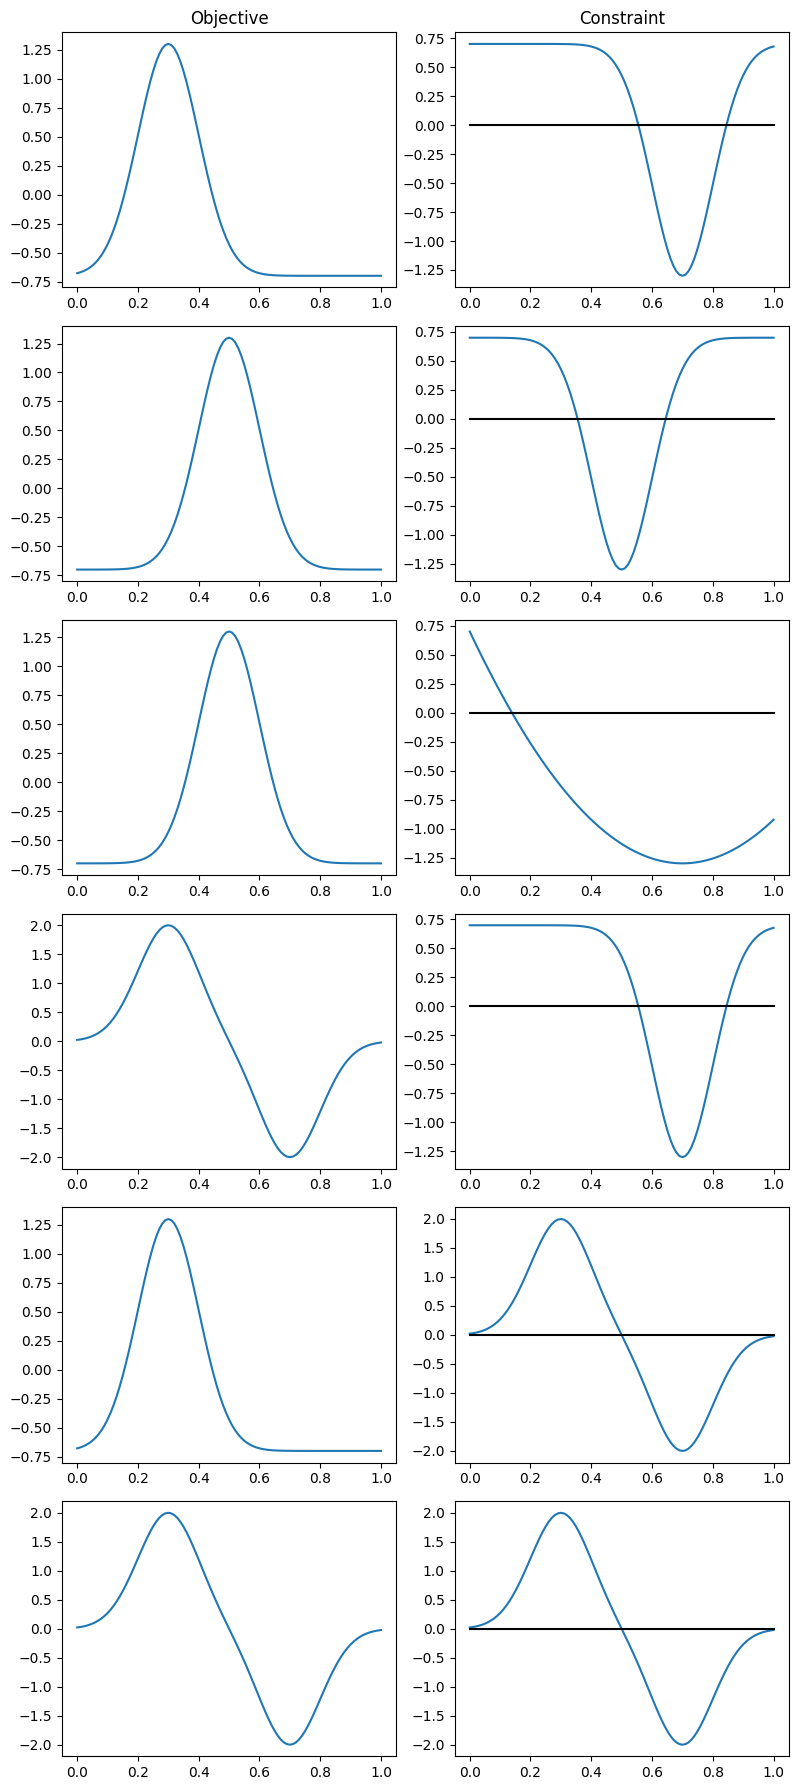
\includegraphics[width=\linewidth, height=20cm]{Figures/toy.png}
    \caption{Toy problems for ablation studies. The region below the black lines are the feasible regions.}
    \label{fig_toy}
\end{figure}

\begin{figure}[h]
    \centering
    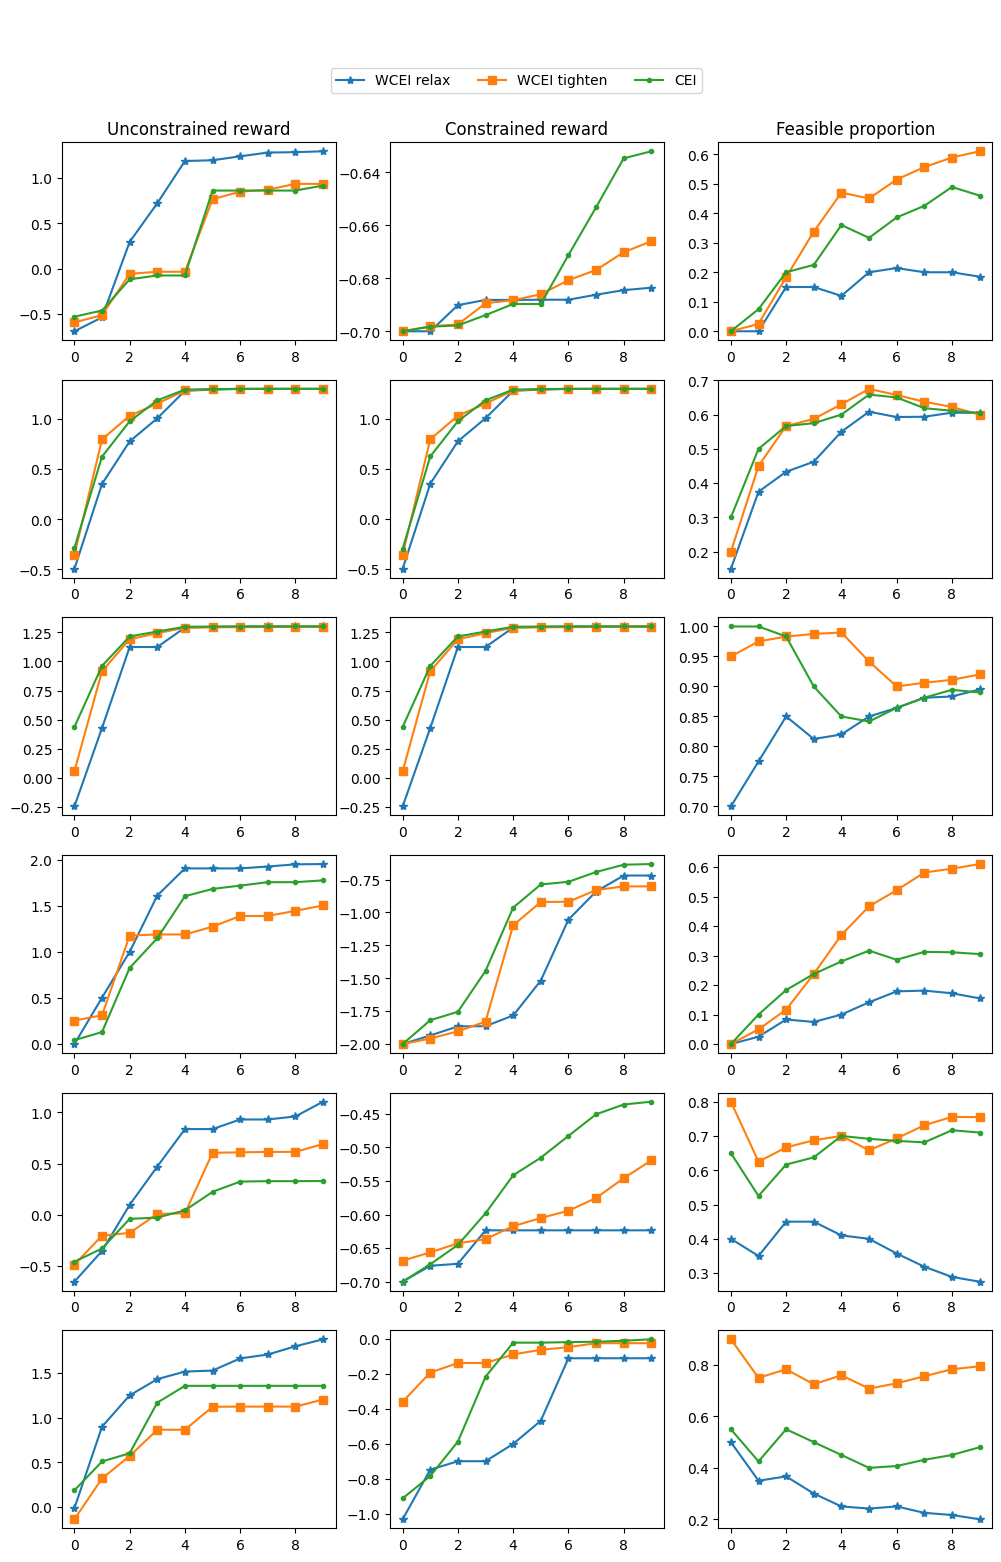
\includegraphics[width=\linewidth, height=20cm]{Figures/toy_res.png}
    \caption{Optimization results for the toy problems. The x axis represent the number of iterations.}
    \label{fig_toy_res}
\end{figure}



\subsection{Simulation study}
In this section, the adaptive policy in Algorithm \ref{algo2} is compared to cEI for the Hartmann6 test function
\begin{align}
    f(x) = -\sum_{i=1}^4\alpha_i\exp{\left(-\sum_{j=1}^6A_{ij}(x_j-P_{ij})^2\right)}
\end{align}
where $x\in[0,1]^6$ and $\alpha_i,A_{ij},P_{ij}$ are known constants. The problem is subjected to the constraint
\begin{align}
    c(x) = \|x\|_1-1.5.
\end{align}
Each method is run for 30 iterations and repeated 20 times. Figure \ref{fig_hart} shows median curves of the runs along with their interquartile range (IQR) for each method. Overall, the adaptive scheme did slightly better than cEI but it is not clear as their IQRs have a lot of overlap.
\begin{figure}[h]
    \centering
    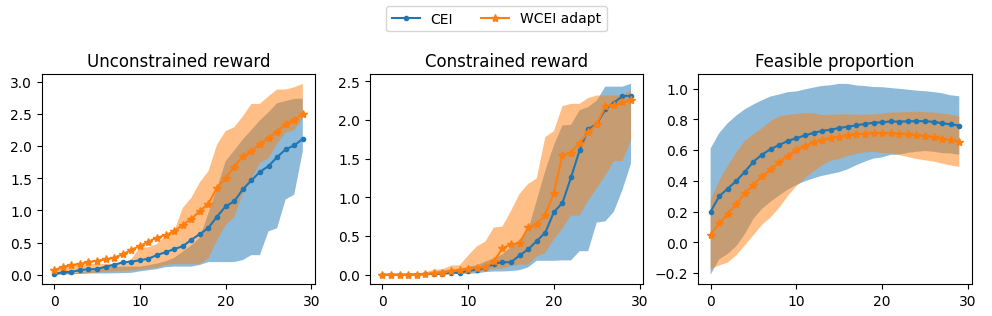
\includegraphics[width=\linewidth]{Figures/hartman_res.png}
    \caption{Optimization results for constrained Hartmann6 problem. The x axis represent the number of iterations.}
    \label{fig_hart}
\end{figure}

\subsection{Discussion}
In this mini-project, I have devised and implemented a new acquisition function for CBO that augments the looseness of the original constrained optimization problem. This class of acquisition functions allows us to construct an adaptive policy that can adjust the level of favoritism for the feasible region. The adaptive policy devised here is relatively primitive and more understanding of WCEI is required to build a more effective policy. Note that this approach of controlling the constraint looseness can also be applied to other methods as well.

The idea of changing the looseness of a CBO problem also have some practical applications. Constraint tightening is beneficial when the constraints must be satisfied to observe the objective such as drug development satisfying safety constraints. On the other hand, in problems such as portfolio building, the budget constraints can be relaxed if it means the expected yield could be significantly improved. 
% ...